%\documentclass[12pt,openright,twoside,a4paper,chapter=TITLE,english]{USPSC}
\documentclass[12pt,openright,twoside,a4paper,english,sumario=tradicional]{USPSC}

% ---
% Pacotes básicos - Fundamentais 
% ---
\usepackage[T1]{fontenc}		% Seleção de códigos de fonte.
\usepackage[utf8]{inputenc}		% Codificação do documento (conversão automática dos acentos)
\usepackage{lmodern}			% Usa a fonte Latin Modern
\usepackage{lastpage}			% Usado pela Ficha catalográfica
\usepackage{indentfirst}		% Indenta o primeiro parágrafo de cada seção.
\usepackage{color}				% Controle das cores
\usepackage{graphicx}			% Inclusão de gráficos
\usepackage{float} 				% Fixa tabelas e figuras no local exato
\usepackage{chemfig,chemmacros} % Para escrever reações químicas
\usepackage{microtype} 			% para melhorias de justificação
\usepackage{pdfpages}
\usepackage{makeidx}            % para gerar índice remissimo

\usepackage[num,overcite,abnt-emphasize=bf, abnt-thesis-year=both, abnt-repeated-author-omit=yes, abnt-last-names=abnt, abnt-etal-cite,abnt-etal-list=0, abnt-etal-text=default, abnt-and-type=e, iso-abbreviation=standard]{abntex2cite}

\renewcommand{\thefootnote}{\fnsymbol{footnote}}  %Comando para inserção de símbolos em nota de rodapé

\renewcommand{\footnotesize}{\small} %Comando para diminuir a fonte das notas de rodapé

\usepackage{cite}	
\usepackage{lipsum}				% para geração de dummy text

% pacotes de tabelas
\usepackage{multicol}	% Suporte a mesclagens em colunas
\usepackage{multirow}	% Suporte a mesclagens em linhas
\usepackage{longtable}	% Tabelas com várias páginas
\usepackage{threeparttablex}    % notas no longtable
\usepackage{array}

%---
% Configurações para o pacote chemfig
%\chemsetup[chemformula]{format=\sffamily}
\renewcommand*\printatom[1]{\ensuremath{\mathsf{#1}}}
\setatomsep{2em}
\setdoublesep{.6ex}
\setbondstyle{semithick}
%---
% Configurando o ambiente para utilizar os recursos de frases pre-prontas do mhchem
\newenvironment{rslist}%
{%
	\begin{labeling}% environment from KOMA-script
		{\rsnumber{R39/23/24/25}}% R39/23/24/25 is longest label
	}{%
\end{labeling}%
}%
% Definição de comando para utilizar os recursos de frases pre-prontas do mhchem
\newcommand{\rs}[2][]{\item[{\rsnumber[#1]{#2}}] \rsphrase{bb}}
% ---

% ---
% DADOS INICIAIS - Define sigla com título, área de concentração e opção do Programa 
% Consulte a tabela referente aos Programas, áreas e opções de sua unidade contante do
% arquivo USPSC-Siglas estabelecidas para os Programas de Pós-Graduação por Unidade.xlsx 
% ou nos APÊNDICES A-G
\siglaunidade{IFSC} 
\programa{DFA}
\definecolor{blue}{RGB}{41,5,195}

% informações do PDF
\makeatletter
\hypersetup{
	%pagebackref=true,
	pdftitle={\@title}, 
	pdfauthor={\@author},
	pdfsubject={\imprimirpreambulo},
	pdfcreator={LaTeX with abnTeX2},
	pdfkeywords={abnt}{latex}{abntex}{USPSC}{trabalho acadêmico}, 
	colorlinks=true,       		% false: boxed links; true: colored links
	linkcolor=blue,          	% color of internal links
	citecolor=blue,        		% color of links to bibliography
	filecolor=magenta,      		% color of file links
	urlcolor=blue,
	bookmarksdepth=4
}
\makeatother
% --- 
% --- 
% Espaçamentos entre linhas e parágrafos 
% --- 

% O tamanho do parágrafo é dado por:
\setlength{\parindent}{1.3cm}

% Controle do espaçamento entre um parágrafo e outro:
\setlength{\parskip}{0.2cm}  % tente também \onelineskip


%%%%%%%%%%%%% RAUL %%%%%%%%%%%%%
\usepackage{cleveref}
\crefname{appendix}{App.}{Apps.}
\crefname{section}{Sec.}{Secs.}
\crefname{paragraph}{Sec.}{Secs.}
\crefname{table}{Tab.}{Tabs.}
\crefname{figure}{Fig.}{Figs.}
\crefname{equation}{Eq.}{Eqs.}
\crefname{item}{item}{items}
\usepackage{xspace}
%\usepackage{enumerate}
\usepackage{enumitem}
\usepackage{amsmath}

%%%%%%% units
\newcommand{\kg}{\ensuremath{\mbox{kg}}\xspace}
\newcommand{\eV}{\ensuremath{\mbox{e\kern-0.1em V}}\xspace}
\newcommand{\EeV}{\ensuremath{\mbox{Ee\kern-0.1em V}}\xspace}
\newcommand{\TeV}{\ensuremath{\mbox{Te\kern-0.1em V}}\xspace}
\newcommand{\PeV}{\ensuremath{\mbox{Pe\kern-0.1em V}}\xspace}
\newcommand{\GeV}{\ensuremath{\mbox{Ge\kern-0.1em V}}\xspace}
\newcommand{\MeV}{\ensuremath{\mbox{Me\kern-0.1em V}}\xspace}
\newcommand{\GeVc}{\ensuremath{\mbox{Ge\kern-0.1em V}\kern-0.1em/\kern-0.05em c}\xspace}
\newcommand{\GeVcc}{\ensuremath{\mbox{Ge\kern-0.1em V}\kern-0.1em/\kern-0.05em c^2}\xspace}
\newcommand{\AGeV}{\ensuremath{A\,\mbox{Ge\kern-0.1em V}}\xspace}
\newcommand{\AGeVc}{\ensuremath{A\,\mbox{Ge\kern-0.1em V}\kern-0.1em/\kern-0.05em c}\xspace}
\newcommand{\MeVc}{\ensuremath{\mbox{Me\kern-0.1em V}\kern-0.1em/\kern-0.05em c}\xspace}
\newcommand{\MeVcc}{\ensuremath{\mbox{Me\kern-0.1em V}\kern-0.1em/\kern-0.05em c^2}\xspace}
\newcommand{\T}{\ensuremath{\mbox{T}}\xspace}
\newcommand{\cmsq}{\ensuremath{\mbox{cm}^2}\xspace}
\newcommand{\msq}{\ensuremath{\mbox{m}^2}\xspace}
\newcommand{\cm}{\ensuremath{\mbox{cm}}\xspace}
\newcommand{\mm}{\ensuremath{\mbox{mm}}\xspace}
\newcommand{\mb}{\ensuremath{\mbox{mb}}\xspace}
\newcommand{\micron}{\ensuremath{\mu\mbox{m}}\xspace}
\newcommand{\mrad}{\ensuremath{\mbox{mrad}}\xspace}
\newcommand{\ns}{\ensuremath{\mbox{ns}}\xspace}
\newcommand{\m}{\ensuremath{\mbox{m}}\xspace}
\newcommand{\s}{\ensuremath{\mbox{s}}\xspace}
\newcommand{\ms}{\ensuremath{\mbox{ms}}\xspace}
\newcommand{\ps}{\ensuremath{\mbox{ps}}\xspace}
\newcommand{\pT}{\ensuremath{p_\text{T}}\xspace}
\newcommand{\pL}{\ensuremath{p_\text{L}}\xspace}
\newcommand{\xF}{\ensuremath{x_\text{F}}\xspace}
\newcommand{\xpF}{\ensuremath{x'_\text{F}}\xspace}
\newcommand{\minv}{\ensuremath{m_\text{inv}}\xspace}

%%%%%%%%%%%%% some software programs and generators
%----- NA61 software
\def\Offline{\mbox{$\overline{\text%
{Off}}$\hspace{.05em}\raisebox{.4ex}{\underline{line}}}\xspace}
\def\SHOE{\mbox{SHO\hspace{-1.34ex}\raisebox{0.2ex}{\color{green}\textasteriskcentered}\hspace{0.25ex}E}\xspace}
\def\DSHACK{\mbox{DS\hspace{0.15ex}$\hbar$ACK}\xspace}
\def\SHINE{\mbox{\textsc{S\hspace{.05em}\raisebox{.4ex}{\underline{hine}}}}\xspace}
%----- event generators
\def\Glissando{\textsc{Glissando}\xspace}
\newcommand{\FlukaLong}{{\scshape Fluka\,2008}\xspace}
\newcommand{\FlukaEleven}{{\scshape Fluka\,2011}\xspace}
\newcommand{\Fluka}{{\scshape Fluka}\xspace}
\newcommand{\UrqmdLong}{{\scshape U}r{\scshape qmd\,1.3.1}\xspace}
\newcommand{\Urqmd}{{\scshape U}r{\scshape qmd}\xspace}
\newcommand{\GheishaLong}{{\scshape Gheisha\,2002}\xspace}
\newcommand{\GheishaOld}{{\scshape Gheisha\,600}\xspace}
\newcommand{\Gheisha}{{\scshape Gheisha}\xspace}
\newcommand{\Corsika}{{\scshape Corsika}\xspace}
\newcommand{\Venus}{{\scshape Venus}\xspace}
\newcommand{\VenusLong}{{\scshape Venus\,4.12}\xspace}
\newcommand{\GiBUU}{{\scshape GiBUU}\xspace}
\newcommand{\GiBUULong}{{\scshape GiBUU\,1.6}\xspace}
\newcommand{\FlukaNewLong}{{\scshape Fluka\,2011.2\_17}\xspace}
\newcommand{\Root}{{\scshape Root}\xspace}
\newcommand{\Geant}{{\scshape Geant}\xspace}
\newcommand{\GeantThree}{{\scshape Geant3}\xspace}
\newcommand{\GeantFour}{{\scshape Geant4}\xspace}
\newcommand{\QGSJet}{{\scshape QGSJet}\xspace}
\newcommand{\DPMJet}{{\scshape DPMJet}\xspace}
\newcommand{\Epos}{{\scshape Epos}\xspace}
\newcommand{\EposLong}{{\scshape Epos\,1.99}\xspace}
\newcommand{\QGSJetLong}{{\scshape QGSJet\,II-04}\xspace}
\newcommand{\QGSJetOldLong}{{\scshape QGSJet\,II-03}\xspace}
\newcommand{\DPMJetLong}{{\scshape DPMJet\,3.06}\xspace}
\newcommand{\SibyllLong}{{\scshape Sibyll\,2.1}\xspace}
\newcommand{\SibyllNewLong}{{\scshape Sibyll\,2.3}\xspace}
\newcommand{\EposLHCLong}{{\scshape Epos\,LHC}\xspace}
\newcommand{\Hsd}{{\scshape Hsd}\xspace}
\newcommand{\Ampt}{{\scshape Ampt}\xspace}

%%%%%%%%%%%%%%%%%%%%%%%% misc
\def\red#1{{\color{red}#1}}
\def\avg#1{\langle{#1}\rangle}
\def\sci#1#2{#1{\times}10^{#2}}
\newcommand{\Fi}[1]{Fig.~\ref{#1}}
\newcommand{\NASixtyOne}{NA61\slash SHINE\xspace}%this seems to work properly to me. aa
\newcommand{\NAFortyNine}{NA49\xspace}%this seems to work properly to me. aa
\newcommand{\CernVM}{\textsc{Cern\-\kern-0.05emVM}\xspace}

%%%%%%%%%%%%%%%%%%%%%%%% RAUL

\newcommand{\E}[1]{$10^{#1}$ \eV\xspace}


\def \nmu{$N_{\mu}$\xspace}
\def \xmax{$X_\text{max}$\xspace}
\def \xmumax{$X^\mu_\text{max}$\xspace}


\def \pions{$\pi^\pm$\xspace}
\def \kaons{K$^\pm$\xspace}
\def \proton{p\xspace}
\def \antiproton{$\bar{\text{p}}$\xspace}
\def \protons{p($\bar{\text{p}}$)\xspace}
\def \lamb{$\Lambda$\xspace}
\def \antilamb{$\bar{\Lambda}$\xspace}
\def \lambs{$\Lambda(\bar{\Lambda})$\xspace}
\def \kzeros{K$_{S}^{0}$\xspace}
\def \pipi{$\pi^+\pi^-$\xspace}
\def \vzero{$V^0$\xspace}
\def \vzeros{$V^0$'s\xspace}


\newcommand{\eps}{\ensuremath{\mbox{$\varepsilon$}}\xspace}
\newcommand{\meaneps}{\ensuremath{\mbox{$\langle\varepsilon\rangle$}}\xspace}
\newcommand{\meanepsbb}{\ensuremath{\mbox{$\langle\varepsilon\rangle^\text{BB}$}}\xspace}
\newcommand{\dedx}{\ensuremath{\mbox{\text{d}$E$/\text{d}$x$}}\xspace}
\newcommand{\ncl}{\ensuremath{\mbox{$n_{\text{cl}}$}}\xspace}
\newcommand{\chisq}{\ensuremath{\mbox{$\chi^2$}}\xspace}
\newcommand{\redchisq}{\ensuremath{\mbox{$\chi^2/$ndf}}\xspace}

\newcommand{\ipart}{\ensuremath{i}\xspace}
\newcommand{\npart}{\ensuremath{I}\xspace}
\newcommand{\ich}{\ensuremath{j}\xspace}
\newcommand{\ieps}{\ensuremath{k}\xspace}
\newcommand{\neps}{\ensuremath{K}\xspace}
%\newcommand{\p}{\ensuremath{p}\xspace}
\newcommand{\iz}{\ensuremath{l}\xspace}
\newcommand{\iq}{\ensuremath{m}\xspace}
\newcommand{\gen}{\text{gen}\xspace}
\newcommand{\sel}{\text{sel}\xspace}
\newcommand{\cmc}{\ensuremath{\mbox{$C_\text{MC}$}}\xspace}

\newcommand{\impact}{\ensuremath{\mbox{$b_r$}}\xspace}
\newcommand{\impactmax}{\ensuremath{\mbox{$b_r^\text{max}$}}\xspace}
\newcommand{\decaydist}{\ensuremath{\mbox{$L_\text{decay}$}}\xspace}
\newcommand{\decaydistmin}{\ensuremath{\mbox{$L_\text{decay}^\text{min}$}}\xspace}



  
  


%aliases for bib entries
\def\NASixtyOnePaper{Abgrall:2014xwa} 
\def\NAFortyNinePaper{Afanasev:1999iu}
\def\T2KPaper{Abe:2011ks}
\def\RhoPaper{Aduszkiewicz:2017anm}
\def\QGSJetPaper{Ostapchenko:2010vb}
\def\DPMJetPaper{Roesler:2000he}
\def\EposPaper{Pierog:2006qv}
\def\EposLHCPaper{Pierog:2013ria}
\def\SibyllPaper{Ahn:2009wx}
\def\NewSibyllPaper{Riehn:2015oba}
\def\APP16{Prado:2016akv}
\def\APP17{Prado:2017ijs}
\def\AlicePaper{Aamodt:2008zz}
\def\CMSPaper{Chatrchyan:2008aa}
\def\IoanaICRC{IoanaICRC2009}
\def\MichaelICRC{UngerICRC2011}
\def\HansICRC{HansICRC2013}
\def\AlexICRC{Herve:2015lra}
\def\RaulICRC{Prado:2017hub}
  



\newcommand{\warning}[1]{\textcolor{red}{\textbf{(#1)}}}
\newcommand{\note}[1]{\textcolor{blue}{\textbf{(#1)}}}
%%%%%%%%%%%%%%%%%%%%%%%%%%%%%%%%




% ---
% compila o sumário e índice
\makeindex
% ---

% ----
% Início do documento
% ----
\begin{document}

% Seleciona o idioma do documento (conforme pacotes do babel)
\selectlanguage{english}

% Retira espaço extra obsoleto entre as frases.
\frenchspacing 

% --- Formatação dos Títulos
\renewcommand{\ABNTEXchapterfontsize}{\fontsize{12}{12}\bfseries}
\renewcommand{\ABNTEXsectionfontsize}{\fontsize{12}{12}\bfseries}
\renewcommand{\ABNTEXsubsectionfontsize}{\fontsize{12}{12}\normalfont}
\renewcommand{\ABNTEXsubsubsectionfontsize}{\fontsize{12}{12}\normalfont}
\renewcommand{\ABNTEXsubsubsubsectionfontsize}{\fontsize{12}{12}\normalfont}


% ----------------------------------------------------------
% ELEMENTOS PRÉ-TEXTUAIS
% ----------------------------------------------------------
% ---
% Capa
% ---
\imprimircapa
% ---
% Folha de rosto
% (o * indica impressão em anverso (frente) e verso )
% ---
\imprimirfolhaderosto*
%\imprimirfolhaderosto
% ---
% ---
% Inserir a ficha catalográfica em pdf
% ---
% A biblioteca da sua Unidade lhe fornecerá um PDF com a ficha
% catalográfica definitiva. 
% Quando estiver com o documento, salve-o como PDF no diretório
% do seu projeto como fichacatalografica.pdf e iclua o arquivo
% utilizando o comando abaixo:
%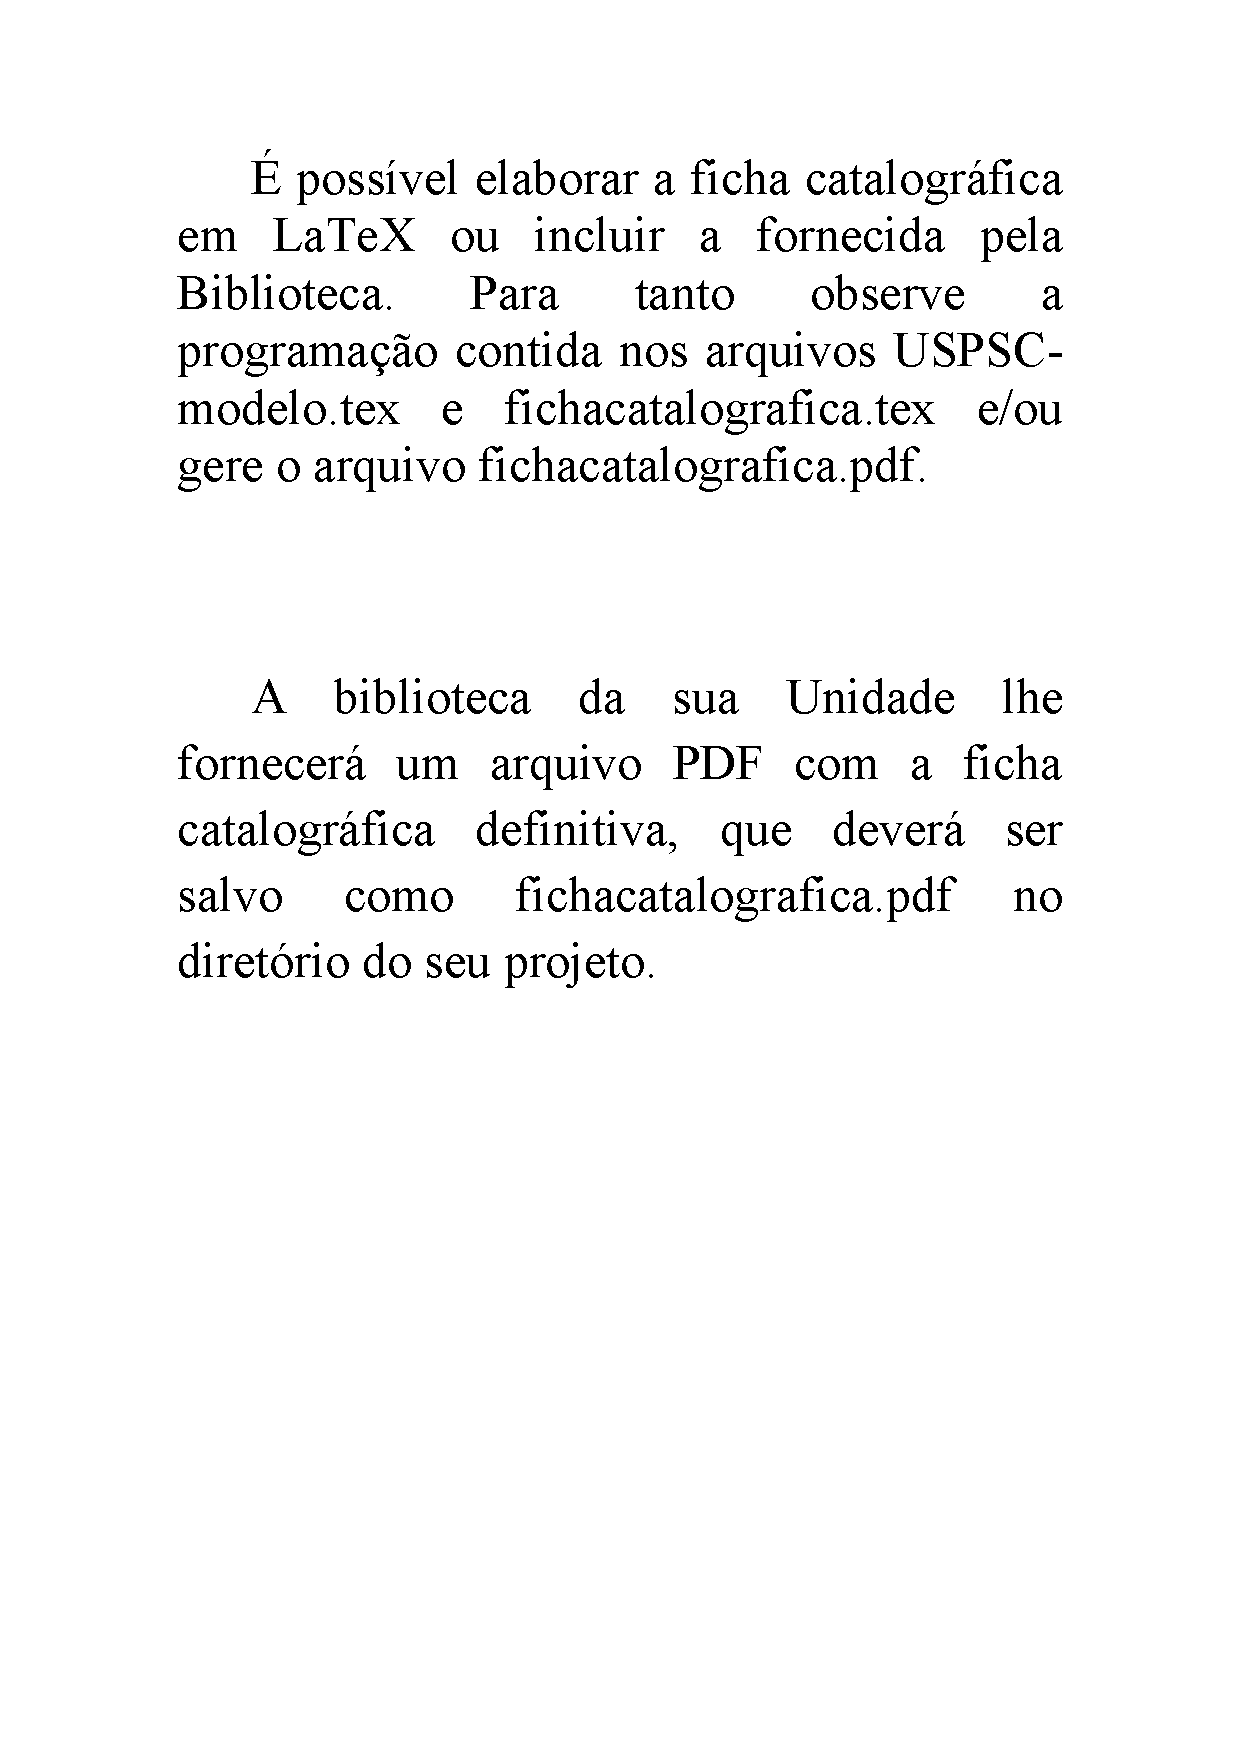
\includepdf{USPSC-Tese-pre-textual/fichacatalografica.pdf} 
% Se você optar por elaborar a ficha catalográfica, deverá 
% incluir uma % antes da linha % antes
% do comando % ---
% Inserir a ficha bibliografica
% ---
% Isto é um exemplo de Ficha Catalográfica, ou ``Dados internacionais de
% catalogação-na-publicação''. Você pode utilizar este modelo como referência. 
% Porém, provavelmente a biblioteca da sua universidade lhe fornecerá um PDF
% com a ficha catalográfica definitiva após a defesa do trabalho. Quando estiver
% com o documento, salve-o como PDF no diretório do seu projeto e substitua todo
% o conteúdo de implementação deste arquivo pelo comando abaixo:
%
\begin{fichacatalografica}
	\hspace{-1.4cm}
	\imprimirnotaautorizacao \\ \\
	%\sffamily
	\vspace*{\fill}					% Posição vertical
	\begin{center}					% Minipage Centralizado
		\imprimirnotabib \\
\begin{table}[htb]
	\scriptsize
	\centering	
	\begin{tabular}{|p{0.9cm} p{8.7cm}|}
		\hline
	      & \\
		  &	  \imprimirautorficha     \\
		
		 \imprimircutter & 
							\hspace{0.4cm}\imprimirtitulo~  / ~\imprimirautor~ ;  ~\imprimirorientadorcorpoficha. -- 	\imprimirlocal, \imprimirdata.   \\
		
		  &  % Para incluir nota referente à versão corrigida no corpo da ficha,
			  % incluir % no início da linha acima e tirar a % do início da linha abaixo
			  %	\hspace{0.4cm} \imprimirtitulo~  / ~\imprimirautor~ ; ~\imprimirorientadorcorpoficha~- ~\imprimirnotafolharosto. -- \imprimirlocal, \imprimirdata.  \\
		
			\hspace{0.4cm}\pageref{LastPage} p. : il. (algumas color.) ; 30 cm.\\ 
		  & \\
		  & 
		    \hspace{0.4cm}\imprimirnotaficha ~--~ 
						  \imprimirunidademin, 
						  \imprimiruniversidademin, 
		                  \imprimirdata. \\ 
		  & \\                 
		   % Para incluir nota referente à versão corrigida em notas,
		    % incluir uma % no início da linha acima e	
		    % tirar a % do início da linha abaixo
		    % & \hspace{0.4cm}\imprimirnotafolharosto \\ 
		  & \\ 
		  & \hspace{0.4cm}1. LaTeX. 2. abnTeX. 3. Classe USPSC. 4. Editoração de texto. 5. Normalização da documentação. 6. Tese. 7. Dissertação. 8. Documentos (elaboração). 9. Documentos eletrônicos. I. \imprimirorientadorficha. 
		   II. Título. \\
	
		     %Se houver co-orientador, inclua % antes da linha (antes de II. Título.) 
		     %          e tire a % antes do comando abaixo 
		     %III. Título. \\   
		  \hline
	\end{tabular}
\end{table}
	\end{center}
\end{fichacatalografica}
% ---

 
% e retirar o % do comando abaixo
%% ---
% Inserir a ficha bibliografica
% ---
% Isto é um exemplo de Ficha Catalográfica, ou ``Dados internacionais de
% catalogação-na-publicação''. Você pode utilizar este modelo como referência. 
% Porém, provavelmente a biblioteca da sua universidade lhe fornecerá um PDF
% com a ficha catalográfica definitiva após a defesa do trabalho. Quando estiver
% com o documento, salve-o como PDF no diretório do seu projeto e substitua todo
% o conteúdo de implementação deste arquivo pelo comando abaixo:
%
\begin{fichacatalografica}
	\hspace{-1.4cm}
	\imprimirnotaautorizacao \\ \\
	%\sffamily
	\vspace*{\fill}					% Posição vertical
	\begin{center}					% Minipage Centralizado
		\imprimirnotabib \\
\begin{table}[htb]
	\scriptsize
	\centering	
	\begin{tabular}{|p{0.9cm} p{8.7cm}|}
		\hline
	      & \\
		  &	  \imprimirautorficha     \\
		
		 \imprimircutter & 
							\hspace{0.4cm}\imprimirtitulo~  / ~\imprimirautor~ ;  ~\imprimirorientadorcorpoficha. -- 	\imprimirlocal, \imprimirdata.   \\
		
		  &  % Para incluir nota referente à versão corrigida no corpo da ficha,
			  % incluir % no início da linha acima e tirar a % do início da linha abaixo
			  %	\hspace{0.4cm} \imprimirtitulo~  / ~\imprimirautor~ ; ~\imprimirorientadorcorpoficha~- ~\imprimirnotafolharosto. -- \imprimirlocal, \imprimirdata.  \\
		
			\hspace{0.4cm}\pageref{LastPage} p. : il. (algumas color.) ; 30 cm.\\ 
		  & \\
		  & 
		    \hspace{0.4cm}\imprimirnotaficha ~--~ 
						  \imprimirunidademin, 
						  \imprimiruniversidademin, 
		                  \imprimirdata. \\ 
		  & \\                 
		   % Para incluir nota referente à versão corrigida em notas,
		    % incluir uma % no início da linha acima e	
		    % tirar a % do início da linha abaixo
		    % & \hspace{0.4cm}\imprimirnotafolharosto \\ 
		  & \\ 
		  & \hspace{0.4cm}1. LaTeX. 2. abnTeX. 3. Classe USPSC. 4. Editoração de texto. 5. Normalização da documentação. 6. Tese. 7. Dissertação. 8. Documentos (elaboração). 9. Documentos eletrônicos. I. \imprimirorientadorficha. 
		   II. Título. \\
	
		     %Se houver co-orientador, inclua % antes da linha (antes de II. Título.) 
		     %          e tire a % antes do comando abaixo 
		     %III. Título. \\   
		  \hline
	\end{tabular}
\end{table}
	\end{center}
\end{fichacatalografica}
% ---


% As informações que compõem a ficha catalográfica estão 
% definidos no arquivo USPSC-pre-textual-UUUU.tex
% ---


% ---
% Inserir folha de aprovação
% ---
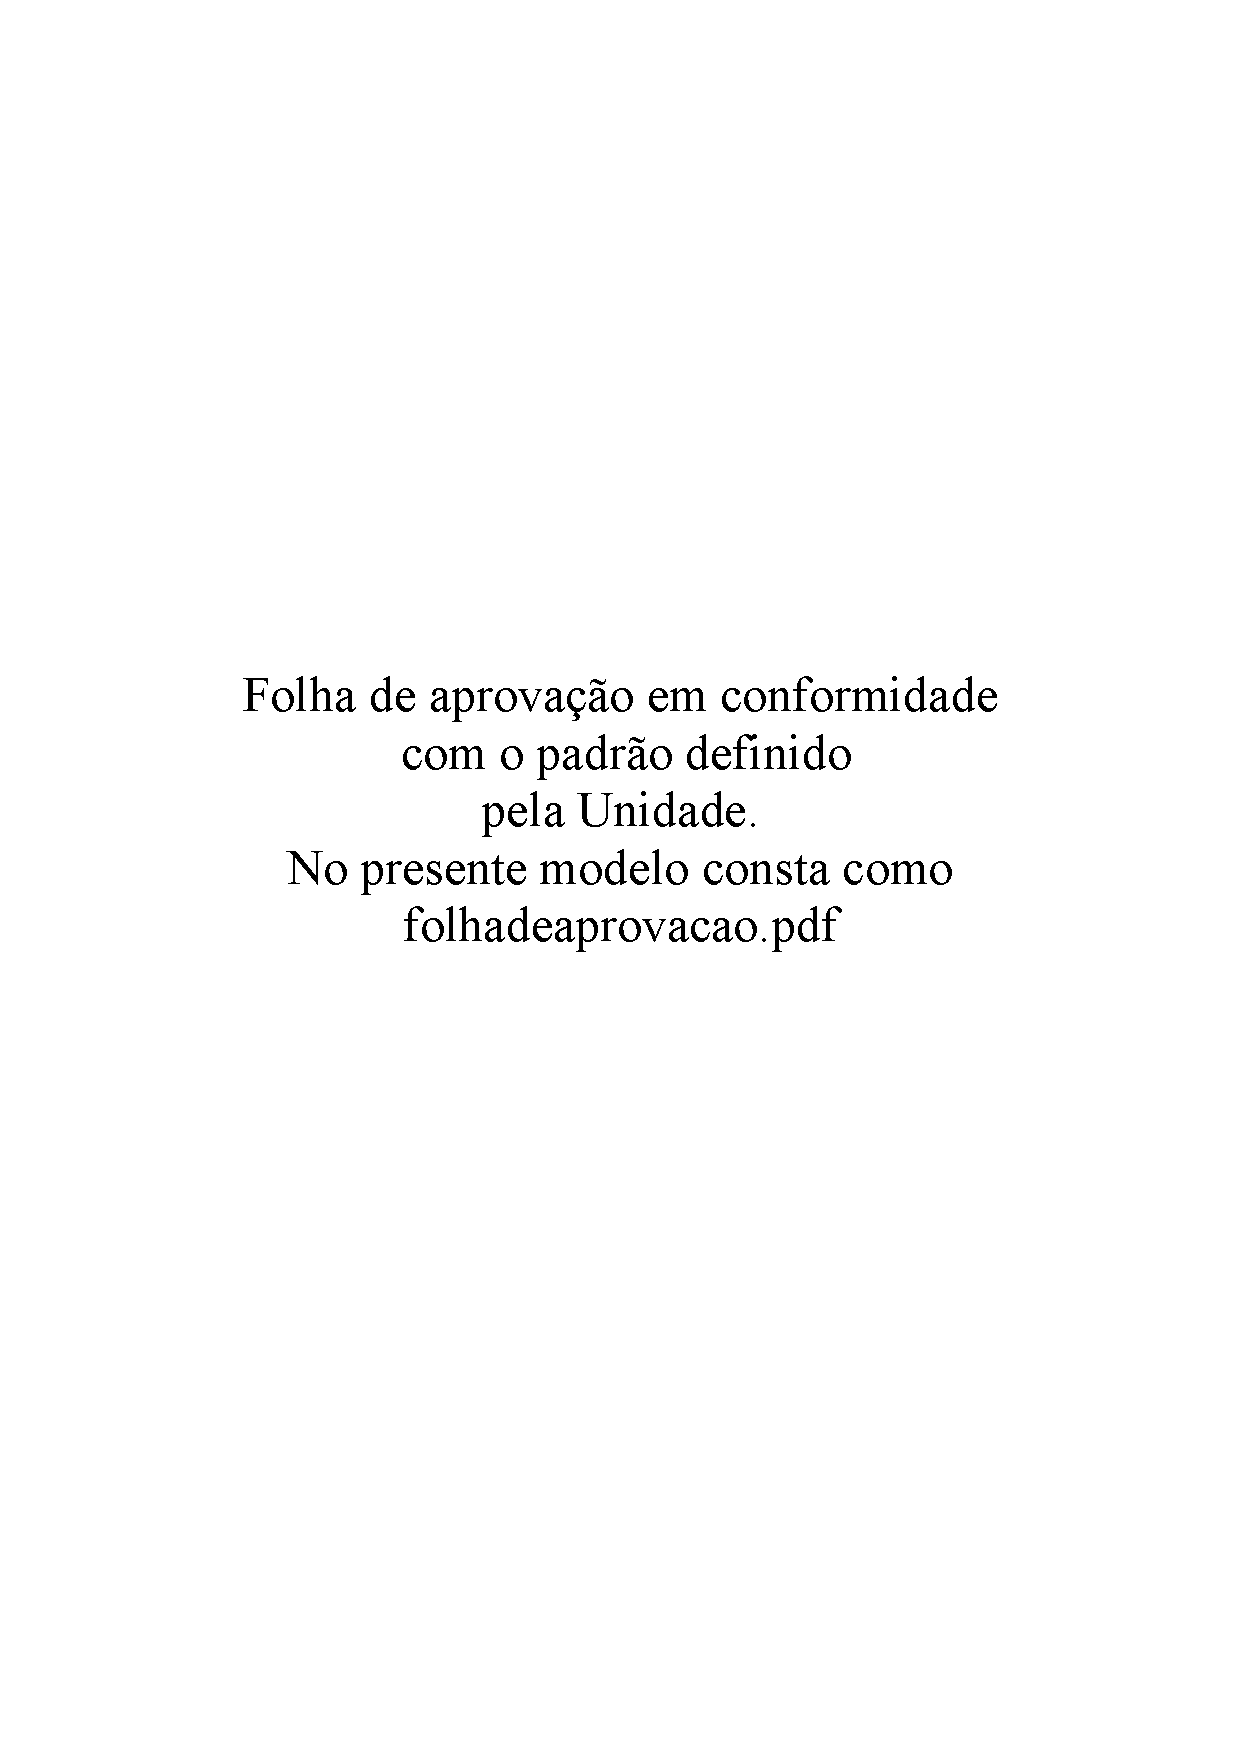
\includepdf{folhadeaprovacao.pdf}


\includepdf{PaginaEmBranco.pdf}

% ---
% Dedicatória
% ---
%\include{USPSC-Dedicatoria}
% ---

% ---
% Agradecimentos
% ---
%% Agradecimentos.tex
% ---
% Agradecimentos
% ---=====
\begin{agradecimentos}
  I am very grateful to:
  \begin{itemize}
  \item
    %\item my advisor Prof. Vitor de Souza;

  %\item the LIP group, in particular to Prof. Mario Pimenta and Ruben Conceição; 

  %\item the KIT group, in particular to Michael Unger, Alex Herve and Darko Veberic; 
    
  %\item my collegues from the Astroparticle Physics group at IFSC;

  %\item family
    
  %\item friend
    
  %\item FAPESP
 
  \end{itemize}

\end{agradecimentos}
% ---

% ---

% ---
% Epígrafe
% ---
\begin{epigrafe}
    \vspace*{\fill}
	\begin{flushright}
		\textit{``O estudo, a busca da verdade e da beleza são domínios \\
		em que nos é consentido sermos crianças por toda a vida.''\\
		Albert Einstein}
	\end{flushright}
\end{epigrafe}
% ---

% A T E N Ç Ã O
% Se o idioma do texto for em inglês, o abstract deve preceder o resumo
% resumo em português
%
% Resumo
% ---
%% Abstract.tex
% ---
% Abstract
% ---
\autor{Prado, R. R.}
\begin{resumo}[Abstract]        
 \begin{otherlanguage*}{english}
	\begin{flushleft} 
		\setlength{\absparsep}{0pt} % ajusta o espaçamento dos parágrafos do resumo		
 		\SingleSpacing 
 		\imprimirautorabr~ ~\textbf{\imprimirtitleabstract}.	\imprimirdata.  \pageref{LastPage}p. 
		%Substitua p. por f. quando utilizar oneside em \documentclass
		%\pageref{LastPage}f.
		\imprimirtipotrabalho~-~\imprimirinstituicao, \imprimirlocal, 	\imprimirdata. 
 	\end{flushleft}
	\OnehalfSpacing 
   This is the english abstract.

   \vspace{\onelineskip}
 
   \noindent 
   \textbf{Keywords}: .
 \end{otherlanguage*}
\end{resumo}

% ---

% Abstract
% ---
%% Resumo.tex
% ---
% Resumo
% ---
\setlength{\absparsep}{18pt} % ajusta o espaçamento dos parágrafos do resumo		
\begin{resumo}[Resumo]
	\begin{flushleft} 
		        \setlength{\absparsep}{0pt} % ajusta o espaçamento da referência	
			\SingleSpacing 
			\imprimirautorabr~ ~\textbf{\imprimirtitleabstract}. \imprimirdata. \pageref{LastPage}p. 
			%Substitua p. por f. quando utilizar oneside em \documentclass
			%\pageref{LastPage}f.
			\imprimirtipotrabalho~-~\imprimirinstituicao, \imprimirlocal, \imprimirdata. 
 	\end{flushleft}
        \OnehalfSpacing 			

Raios C\'osmicos Ultra Energ\'eticos (Ultra-High Energy Cosmic Rays, UHECR) somente
podem ser medidos atrav\'es da detec\c{c}\~ao dos Chuveiros Atmosf\'ericos Extensos
(Extensive Air Showers, EAS) criados pela intera\c{c}\~ao do raio c\'osmico prim\'ario com
n\'ucleos atmof\'ericos. A infer\^encia de algumas propriedados dos UHECRs, como a composi\c{c}\~ao
de massa, \'e poss\'ivel somente atrav\'es da compara\c{c}\~ao entre medidas de observ\'aveis dos EASs
com predi\c{c}\~oes geradas por simula\c{c}\~oes de Monte Carlo. A fonte de incerteza mais importante
na descri\c{c}\~ao de EAS por simula\c{c}\~oes \'e a modelagem das intera\c{c}\~oes hadr\^onicas. Por muitos
anos \'e sabido que os modelos de intera\c{c}\~ao hadr\^onica falham na predi\c{c}\~ao de observ\'aveis
dos EASs relacionados a sua componente mu\^onica. A manifesta\c{c}\~ao mais evidente disso \'e 
chamada \emph{problema do d\'eficit de m\'uons} devido ao fato que o n\'umero de m\'uons em chuveiros
com energies acima de \E{18} predito por simula\c{c}\~oes \'e menor que os observados.
O objetivo desta tese \'e abordar este problema atrav\'es de tr\^es frentes. Primeiramente,
um m\'etodo \'e desenvolvido para interpretar as medidas do n\'umero de muons em termos
de composi\c{c}\~ao de raios c\'osmicos considerando o problema do d\'eficit de m\'uons.
Segundo, a proposta e o teste de um observ\'avel que \'e sens\'ivel ao espectro de energia dos m\'uons
na superf\'icie e, consequentemente, pode ser usado para constrair os modelos de intera\c{c}\~ao hadr\^onica.
Por \'ultima, a produ\c{c}\~ao de m\'uons em chuveiros \'e estudada atrav\'es
de medidas do espectro de produ\c{c}\~ao de hadrons em intera\c{c}\~oes do tipo p\'ion-carbono.



 \textbf{Palavras-chave}: Raios c\'osmicos de altas energies. Chuveiros atmsf\'ericos extensos. Componente mu\^onica de chuveiros atmosf\'ericos. F\'isica de chuveiros atmosf\'ericos.   
\end{resumo}

% ---

% ---
% inserir lista de figurass
% ---
\pdfbookmark[0]{\listfigurename}{lof}
\listoffigures*
\cleardoublepage
% ---

% ---
% inserir lista de tabelas
% ---
\pdfbookmark[0]{\listtablename}{lot}
\listoftables*
\cleardoublepage
% ---

% ---
% inserir lista de quadros
% ---
%\pdfbookmark[0]{\listofquadroname}{loq}
%\listofquadro*
%\cleardoublepage
% ---

% ---
% inserir lista de abreviaturas e siglas
% ---
%\begin{siglas}
%    \item[ABNT] Associação Brasileira de Normas Técnicas
%    \item[abnTeX] ABsurdas Normas para TeX
%	\item[EESC] Escola de Engenharia de São Carlos
%	\item[IAU] Instituto de Arquitetura e Urbanismo
%	\item[IBGE] Instituto Brasileiro de Geografia e Estatística
%	\item[ICMC] Instituto de Ciências Matemáticas e de Computação
%	\item[IFSC] Instituto de Física de São Carlos
%	\item[IQSC] Instituto de Química de São Carlos
%	\item[PDF] Portable Document Format
%	\item[TCC] Trabalho de Conclusão de Curso
%	\item[USP] Universidade de São Paulo
%	\item[USPSC] Campus USP de São Carlos
%\end{siglas}
% ---

% ---
% inserir lista de símbolos
% ---
%\begin{simbolos}
%  \item[$ \Gamma $] Letra grega Gama
%  \item[$ \Lambda $] Lambda
%  \item[$ \zeta $] Letra grega minúscula zeta
%  \item[$ \in $] Pertence
%\end{simbolos}
% ---
% ---
% inserir o sumario
% ---
\pdfbookmark[0]{\contentsname}{toc}
\tableofcontents*
\cleardoublepage
% ---
% ----------------------------------------------------------
% ELEMENTOS TEXTUAIS
% ----------------------------------------------------------
\textual

\chapter[Introduction]{Introduction}
\label{sec:introduction}

The Earth is constantly being reached by charged particles
coming from extraterrestrial sources, which are called Cosmic Rays.
For over a century, the study of these particles have been a very active field
that integrates aspects from both particle physics and astrophysics.
The extremelly wide energy range covered by the well know cosmic rays
energy spectrum make clear that a number of different astrophysical phenomena,
at distinct scales, are contributing to the production of these particles.

Of particular interest is the ultra-high energy range that includes
particles from $E=\E{17}$ up the end of the spectrum at $\sim\E{20.5}$. 
Althought the existence of these ultra-high energy particles is known
since the 1960's, due to detections done by Haverah Park experiment,
the precise measurements of their energy spectra and other features
became possible after the 1990's, with the experiments Fly's Eyes,
HiRes and AGASA. During the last decade, two modern experiments have
been running at the ultra-high energy range, Pierre Auger Observatory
and Telescope Array. 
Even though a large number of important results have been provided
by these experiments lately, the main question about the origin
of ultra-high energy cosmic rays are still unsolved. 
Apart from knowing the astrophysical sources and the acceleration
mechanisms, it is also unclear what is the exact nature of two evident structures
observed in the ultra-high energy spectrum, the \emph{ankle} and the \emph{suppression}.




Because of the very low flux of particles at the 



The compreesion of the astrophysical aspects behind the cosmic rays
is mainly complicated by the fact that they cannot be directly measured
at the high energy regime. Their detection is actually done by measuring
the cascade of particles created by the interaction of the cosmic ray particle
with atmospheric nuclei, the so called \emph{Extensive Air Showers}.  


Thus, the properties of the primary particles have to be infered from


The inferences of the properties of the primary cosmic ray have then
to be done by means of the measured features of the 





-cosmic rays->uhe->open questions

-cr->showers->understanding to infer

-muons->muon deficit problem

-augerprime->chap 3 and 4->simulation studies

-na61->pion-air








\chapter[Extensive air showers]{Extensive air showers}
\label{sec:showers}


\section{Particle production}


\section{Observables}





\chapter[Pierre Auger Observatory]{Pierre Auger Observatory}
\label{sec:auger}


\chapter[\NASixtyOne experiment]{\NASixtyOne experiment}
\label{sec:shine}


\chapter[Interpretation of measurements of the number of muons in extensive air shower experiments]{Interpretation of measurements of the number of muons in extensive air shower experiments}
\label{sec:interpretation}

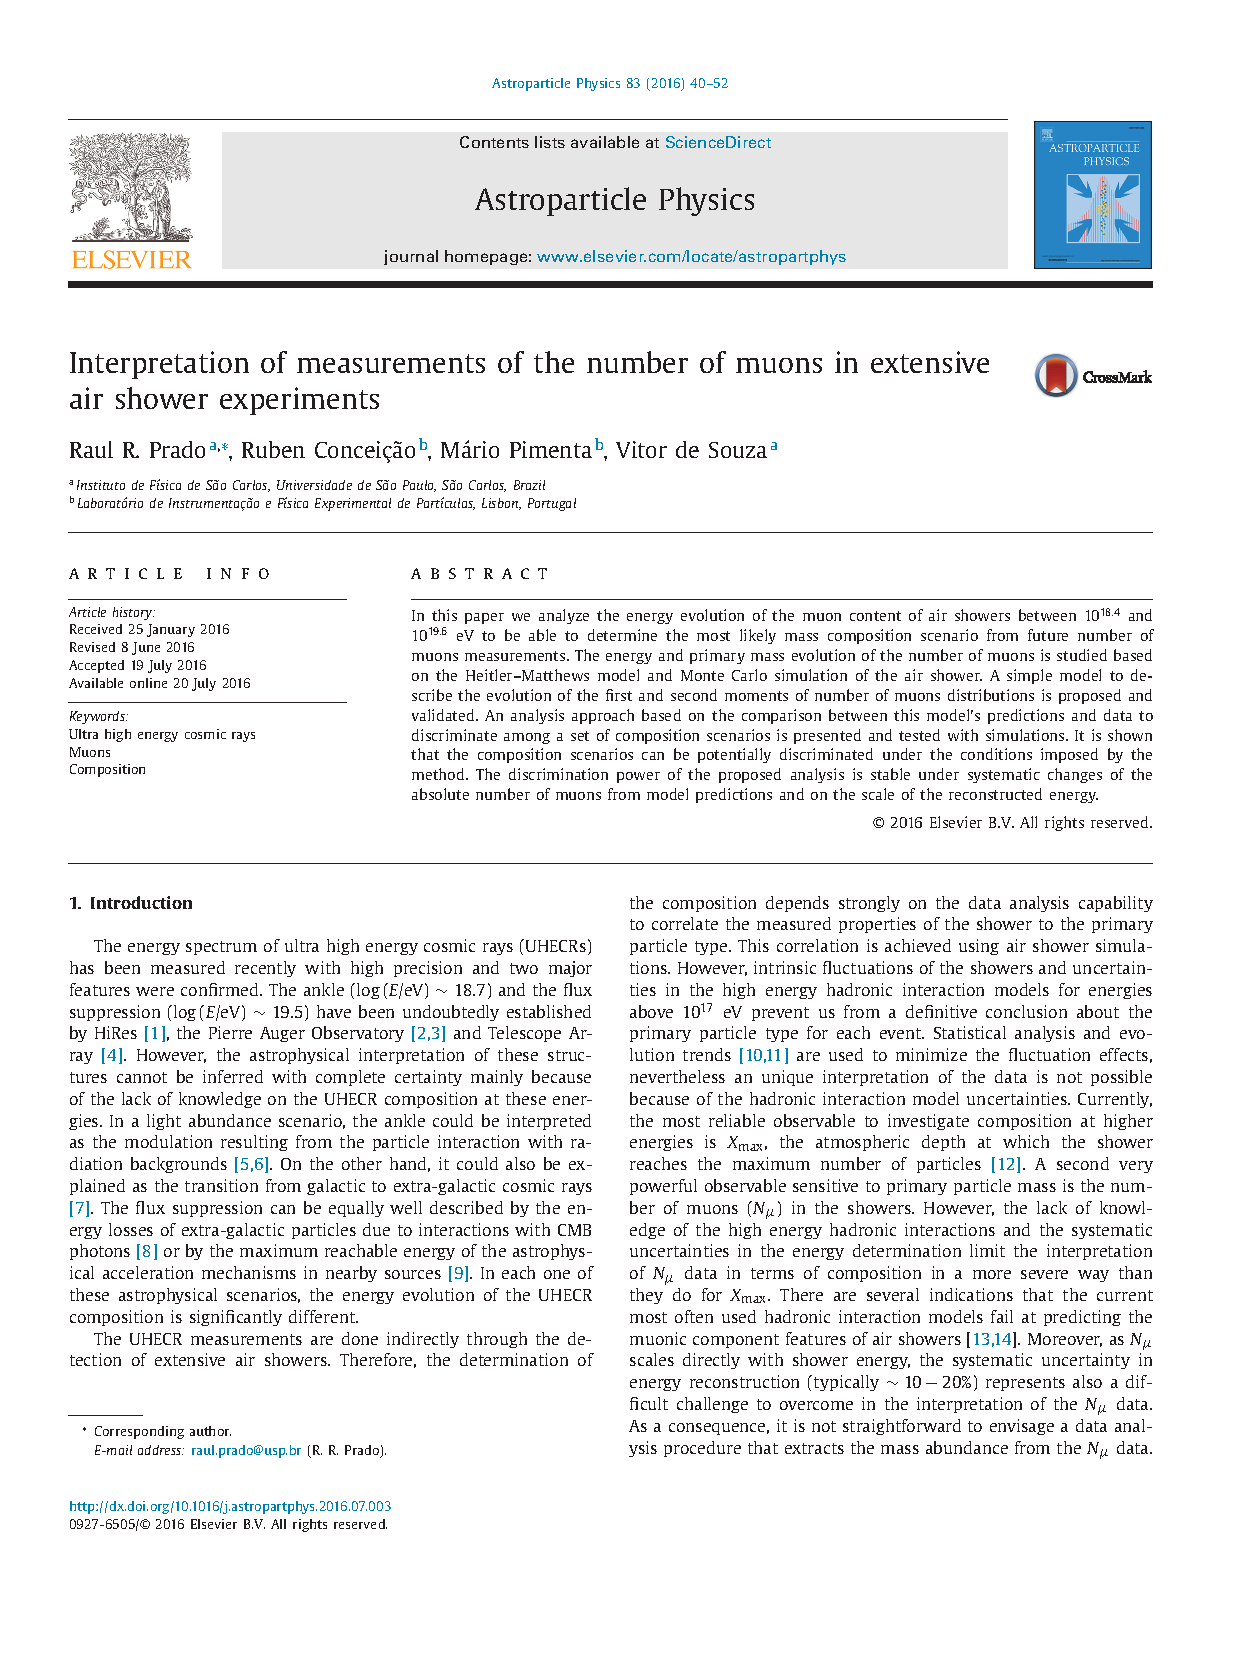
\includepdf[pages=-]{paper_interpretation.pdf}




\chapter[A new air-shower observable to constrain hadronic interaction models]{A new air-shower observable to constrain hadronic interaction models}
\label{sec:observable}

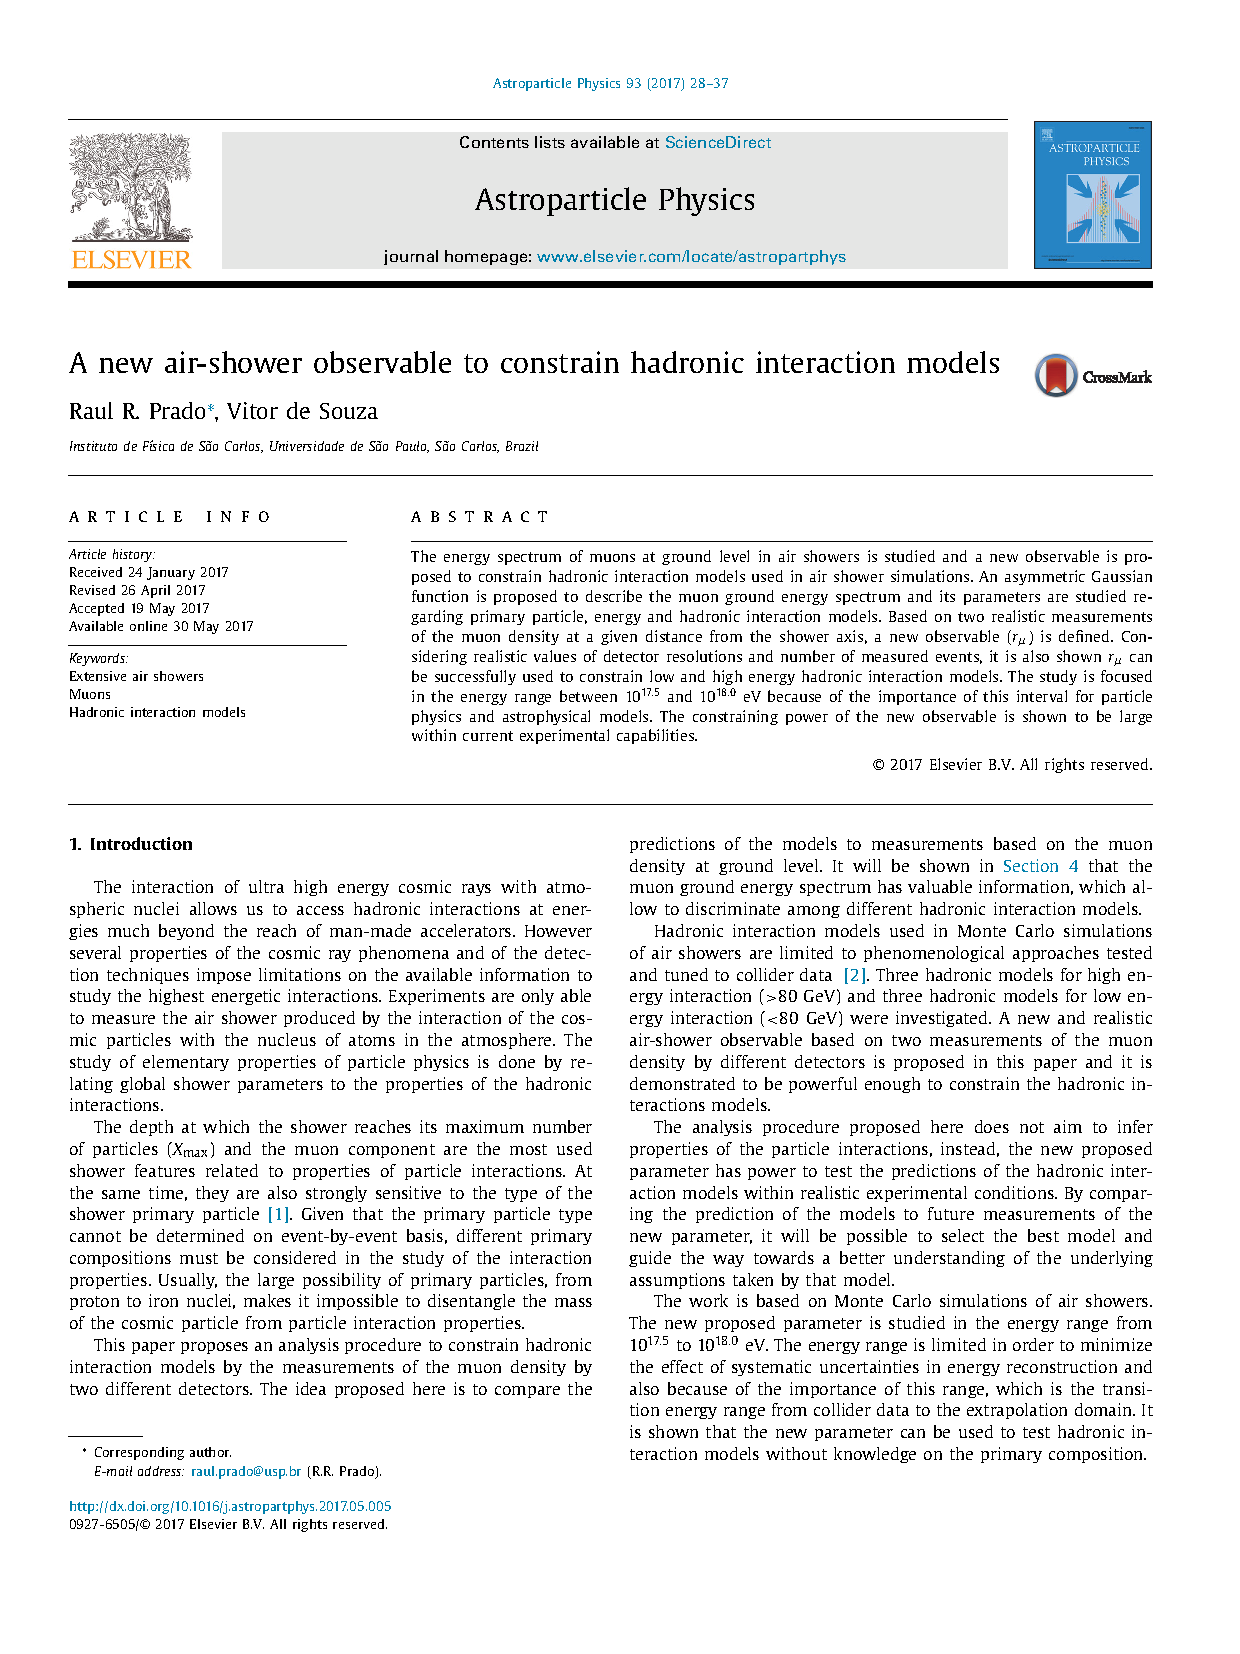
\includepdf[pages=-, pagecommand={}]{paper_observable.pdf}



\chapter[Hadron production in pion-carbon interactions]{Hadron production in pion-carbon interactions}
\label{sec:hadron}


\cite{\NASixtyOnePaper}

\cite{\NAFortyNinePaper}

\cite{\RhoPaper}

\cite{\ICRC17}

%\cite{\APP17}

%\cite{\APP16}

\cite{\QGSJetPaper}

\cite{\DPMJetPaper}

\cite{\EposPaper}



\chapter[Conclusions]{Conclusions}
\label{sec:conclusions}



% ----------------------------------------------------------
% ELEMENTOS PÓS-TEXTUAIS
% ----------------------------------------------------------
\postextual
% ----------------------------------------------------------

% -----------------------------------------------------------
% Referências bibliográficas
% ----------------------------------------------------------
\bibliography{lib}


% ----------------------------------------------------------
% Glossário
% ----------------------------------------------------------
%
% Consulte o manual da classe abntex2 para orientações sobre o glossário.
%
%\glossary

% ----------------------------------------------------------
% Apêndices
% ----------------------------------------------------------
%%% USPSC-Apendice.tex
% ---
% Inicia os apêndices
% ---

\begin{apendicesenv}
% Imprime uma página indicando o início dos apêndices
\partapendices
\chapter{Apendice(s)}
Elemento opcional, que consiste em texto ou documento elaborado pelo autor, a fim de complementar sua argumentação, conforme a ABNT NBR 14724 \cite{nbr14724}.

Os apêndices devem ser identificados por letras maiúsculas consecutivas, seguidas de hífen e pelos respectivos títulos. Excepcionalmente, utilizam-se letras maiúsculas dobradas na identificação dos apêndices, quando esgotadas as 26 letras do alfabeto. A paginação deve ser contínua, dando seguimento ao texto principal. \cite{sibi2009}.

\chapter{Siglas dos Programas de Pós-Graduação da EESC}
\index{quadros}O \autoref{quadro-eesc} relaciona as siglas estabelecidas para os programas de pós-graduação da EESC.

\begin{quadro}[htb]
\ABNTEXfontereduzida
%\caption[Siglas dos Programas de Pós-Graduação da EESC]{Siglas dos Programas de Pós-Graduação da EESC]{Siglas dos Programas de Pós-Graduação da EESC}
\caption[Siglas dos Programas de Pós-Graduação da EESC]{Siglas dos Programas de Pós-Graduação da EESC} 
\label{quadro-eesc}
\begin{tabular}{|p{6.0cm}|p{4.5cm}|p{2.0cm}|p{1.75cm}|}
%\multicolumn{4}{c}%
%{{\tablename\ \thetable{} -- Siglas dos Programas de Pós-Graduação da EESC}} \\
\multicolumn{4}{r}{{(continua)}} \\ 
  \hline
   \textbf{PROGRAMA} & \textbf{ÁREA DE CONCENTRAÇÃO} & \textbf{TÍTULO} & \textbf{SIGLA}  \\
    \hline
Programa de Pós-Graduação em Ciências da Engenharia Ambiental & Ciências da Engenharia Ambiental & Doutor & DCEA \\
Programa de Pós-Graduação em Ciências da Engenharia Ambiental & Ciências da Engenharia Ambiental & Mestre & MCEA \\
Programa de Pós-Graduação em Ciência e Engenharia de Materiais & Desenvolvimento, Caracterização e Aplicação de Materiais  & Doutor & DCEM \\
Programa de Pós-Graduação em Ciência e Engenharia de Materiais & Desenvolvimento, Caracterização e Aplicação de Materiais & Mestre & MCEM \\
Programa de Pós-Graduação em Engenharia Civil (Engenharia de Estruturas) & Estruturas & Doutor & DEE \\
Programa de Pós-Graduação em Engenharia Civil (Engenharia de Estruturas) & Estruturas & Mestre & MEE \\
Programa de Pós-Graduação em Engenharia de Produção & Economia, Organizações e Gestão do Conhecimento & Doutor & DEPE \\
Programa de Pós-Graduação em Engenharia de Produção & Economia, Organizações e Gestão do Conhecimento & Mestre & MEPE \\
Programa de Pós-Graduação em Engenharia de Produção & Processos e Gestão de Operações & Doutor & DEPP \\
Programa de Pós-Graduação em Engenharia de Produção & Processos e Gestão de Operações & Mestre & MEPP \\
Programa de Pós-Graduação em Engenharia de Transportes & Infraestrutura de Transportes & Doutor & DETI \\
Programa de Pós-Graduação em Engenharia de Transportes & Infraestrutura de Transportes & Mestre & METI \\
Programa de Pós-Graduação em Engenharia de Transportes & Planejamento e Operação de Sistemas de Transporte & Doutor & DETP \\
Programa de Pós-Graduação em Engenharia de Transportes & Planejamento e Operação de Sistemas de Transporte & Mestre & METP \\
Programa de Pós-Graduação em Engenharia de Transportes & Transportes & Doutor & DETT \\
Programa de Pós-Graduação em Engenharia de Transportes & Transportes & Mestre & METT \\
Programa de Pós-Graduação em Engenharia Elétrica & Processamento de Sinais e Intrumentação & Doutor & DEEP \\

\end{tabular}
\end{quadro} 

% o comando \clearpage é necessário para deixar o final da tabela o topo da página, sem ele o final da tabela é centralizado verticalmente na página 
\clearpage
\begin{quadro}[htb]
	\ABNTEXfontereduzida
\begin{tabular}{|p{6.0cm}|p{4.5cm}|p{2.0cm}|p{1.75cm}|}	
 \multicolumn{4}{c}%
	{{\quadroname\ \thequadro{} -- Siglas dos Programas de Pós-Graduação da EESC}} \\
	\multicolumn{4}{r}{{(continuação)}} \\
	 \hline
   \textbf{PROGRAMA} & \textbf{ÁREA DE CONCENTRAÇÃO} & \textbf{TÍTULO} & \textbf{SIGLA}  \\
		 \hline
Programa de Pós-Graduação em Engenharia Elétrica & Processamento de Sinais e Intrumentação & Mestre & MEEP \\
Programa de Pós-Graduação em Engenharia Elétrica & Sistemas Dinâmicos & Doutor & DEED \\
Programa de Pós-Graduação em Engenharia Elétrica & Sistemas Dinâmicos & Mestre & MEED \\
Programa de Pós-Graduação em Engenharia Elétrica & Sistemas Elétricos de Potência & Doutor & DEEE \\
Programa de Pós-Graduação em Engenharia Elétrica & Sistemas Elétricos de Potência & Mestre & MEEE \\
Programa de Pós-Graduação em Engenharia Elétrica & Telecomunicações & Doutor & DEET \\
Programa de Pós-Graduação em Engenharia Elétrica & Telecomunicações & Mestre & MEET \\
Programa de Pós-Graduação em Engenharia Hidráulica e Saneamento & Hidráulica e Saneamento & Doutor & DEHS \\
Programa de Pós-Graduação em Engenharia Hidráulica e Saneamento & Hidráulica e Saneamento & Mestre & MEHS \\
Programa de Pós-Graduação em Engenharia Mecânica & Aeronaves & Doutor & DEMA \\
Programa de Pós-Graduação em Engenharia Mecânica & Aeronaves & Mestre & MEMA \\
Programa de Pós-Graduação em Engenharia Mecânica & Dinâmica das Máquinas e Sistemas & Doutor & DEMD \\
Programa de Pós-Graduação em Engenharia Mecânica & Dinâmica das Máquinas e Sistemas & Mestre & MEMD \\
Programa de Pós-Graduação em Engenharia Mecânica & Manufatura & Doutor & DEMF \\
Programa de Pós-Graduação em Engenharia Mecânica & Manufatura & Mestre & MEMF \\
Programa de Pós-Graduação em Engenharia Mecânica & Materiais & Doutor & DEMT \\
Programa de Pós-Graduação em Engenharia Mecânica & Materiais & Mestre & MEMT \\
Programa de Pós-Graduação em Engenharia Mecânica & Projeto Mecânico & Doutor & DEMP \\
Programa de Pós-Graduação em Engenharia Mecânica & Projeto Mecânico & Mestre & MEMP \\
Programa de Pós-Graduação em Engenharia Mecânica & Térmica e Fluídos & Doutor & DEML \\
Programa de Pós-Graduação em Engenharia Mecânica & Térmica e Fluídos & Mestre & MEML \\
Programa de Pós-Graduação em Geotecnia & Geotecnia & Doutor & DGEO \\
Programa de Pós-Graduação em Geotecnia & Geotecnia & Mestre & MGEO \\
    
\end{tabular}
\end{quadro}

% o comando \clearpage é necessário para deixar o final da tabela o topo da página, sem ele o final da tabela é centralizado verticalmente na página 
\clearpage
\begin{quadro}[htb]
	\ABNTEXfontereduzida
\begin{tabular}{|p{6.0cm}|p{4.5cm}|p{2.0cm}|p{1.75cm}|}
\multicolumn{4}{c}%
	{{\quadroname\ \thequadro{} -- Siglas dos Programas de Pós-Graduação da EESC}} \\
	\multicolumn{4}{r}{{(conclusão)}} \\
\hline
\textbf{PROGRAMA} & \textbf{ÁREA DE CONCENTRAÇÃO} & \textbf{TÍTULO} & \textbf{SIGLA}  \\
\hline    
Programa de Pós-Graduação Interunidades em Bioengenharia & Bioengenharia & Doutor & DIUB \\
Programa de Pós-Graduação Interunidades em Bioengenharia & Bioengenharia & Mestre & MIUB \\
Programa de Pós-Graduação em Rede Nacional para Ensino das Ciências Ambientais & Ensino de Ciências Ambientais & Mestre & MRNECA \\    
    
    \hline
\end{tabular}
\begin{flushleft}
		Fonte: Elaborado pelos autores.\
\end{flushleft}
\end{quadro}

% ----------------------------------------------------------
\chapter{Siglas dos Programas de Pós-Graduação do IAU}
\index{quadros}O \autoref{quadro-iau} relaciona as siglas estabelecidas para os programas de pós-graduação do IAU.
\begin{quadro}[htb]
\ABNTEXfontereduzida
\caption[Siglas dos Programas de Pós-Graduação do IAU]{Siglas dos Programas de Pós-Graduação do IAU}
\label{quadro-iau}
\begin{tabular}{|p{3.5cm}|p{3.5cm}|p{3.5cm}|p{1.5cm}|p{2.25cm}|}
  \hline
   \textbf{PROGRAMA} & \textbf{ÁREA DE CONCENTRAÇÃO} & \textbf{OPÇÃO} & \textbf{TÍTULO} & \textbf{SIGLA}  \\
    \hline
Programa de Pós-Graduação em Arquitetura e Urbanismo & Arquitetura, Urbanismo e Tecnologia &  & Doutor & DAUT\\
Programa de Pós-Graduação em Arquitetura e Urbanismo & Arquitetura, Urbanismo e Tecnologia &  & Mestre & MAUT\\
Programa de Pós-Graduação em Arquitetura e Urbanismo & Teoria e História da Arquitetura e do Urbanismo &  & Doutor & DAUH\\
Programa de Pós-Graduação em Arquitetura e Urbanismo & Teoria e História da Arquitetura e do Urbanismo &  & Mestre & MAUH\\
    \hline

\end{tabular}
\begin{flushleft}
		Fonte: Elaborado pelos autores.\
\end{flushleft}
\end{quadro}

% ----------------------------------------------------------
\chapter{Siglas dos Programas de Pós-Graduação do ICMC}
\index{quadros}O \autoref{quadro-icmc} relaciona as siglas estabelecidas para os programas de pós-graduação do ICMC.
\begin{quadro}[htb]
\ABNTEXfontereduzida
\caption[Siglas dos Programas de Pós-Graduação do ICMC]{Siglas dos Programas de Pós-Graduação do ICMC}
\label{quadro-icmc}
\begin{tabular}{|p{3.5cm}|p{3.5cm}|p{3.5cm}|p{1.5cm}|p{2.25cm}|}
  \multicolumn{5}{r}{{(continua)}} \\ 
  \hline
   \textbf{PROGRAMA} & \textbf{ÁREA DE CONCENTRAÇÃO} & \textbf{OPÇÃO} & \textbf{TÍTULO} & \textbf{SIGLA}  \\
    \hline
		Ciências de Computação e Matemática Computacional	& Ciências de Computação e Matemática Computacional	&   &	Doutor	 & DCCp\\
    Ciências de Computação e Matemática Computacional	& Ciências de Computação e Matemática Computacional	&   &	Mestre	& MCCp\\
		Computer Science and Computational Mathematics & Computer Science and Computational Mathematics	&   &	Doctorate & DCCe\\
		Doctorate Program in Mathematics & Mathematics &   &	Doctorate & DMAe\\
		Interinstitucional de Pós-Graduação em Estatística & Estatística &  & Doutor	 & DESp\\
		Interinstitucional de Pós-Graduação em Estatística & Estatística &  & Mestre & MESp\\
		Join Graduate Program in Statistics & Computer Science and Computational Mathematics &  & Master & MCCe\\
		Join Graduate Program in Statistics & Statistics &  & Doctorate & 	DESe\\
    Join Graduate Program in Statistics & Statistics &  & Master & MESe\\
		Master Program in Mathematics &	Mathematics &  & Master &	MMAe\\
		Mathematics Professional Master\'{}s Program &	Mathematics &	 & Master &	MPMe\\
		Programa de Mestrado Profissional em Matemática & Matemática &  & Mestre & MPMp\\
		\end{tabular}
\end{quadro}

% o comando \clearpage é necessário para deixar o final da tabela o topo da página, sem ele o final da tabela é centralizado verticalmente na página 
\clearpage
\begin{quadro}[htb]
\ABNTEXfontereduzida
\begin{tabular}{|p{3.5cm}|p{3.5cm}|p{3.5cm}|p{1.5cm}|p{2.25cm}|}
	\multicolumn{5}{c}%
	{{\quadroname\ \thequadro{} -- Siglas dos Programas de Pós-Graduação do ICMC}} \\
	\multicolumn{5}{r}{{(conclusão)}} \\
	\hline
   \textbf{PROGRAMA} & \textbf{ÁREA DE CONCENTRAÇÃO} & \textbf{OPÇÃO} & \textbf{TÍTULO} & \textbf{SIGLA}  \\	
	 \hline
  	Programa de Pós-Graduação em Matemática & Matemática &  & Doutor & DMAp\\
		Programa de Pós-Graduação em Matemática & Matemática &  & Mestre & MMAp\\
    \hline

\end{tabular}
\begin{flushleft}
		Fonte: Elaborado pelos autores.\
\end{flushleft}
\end{quadro}

% ----------------------------------------------------------
\chapter{Siglas dos Programas de Pós-Graduação do IFSC}
\index{quadros}O \autoref{quadro-ifsc} relaciona as siglas estabelecidas para os programas de pós-graduação do IFSC.
\begin{quadro}[htb]
\ABNTEXfontereduzida
\caption[Siglas dos Programas de Pós-Graduação do IFSC]{Siglas dos Programas de Pós-Graduação do IFSC}
\label{quadro-ifsc}
\begin{tabular}{|p{3.5cm}|p{3.5cm}|p{3.5cm}|p{1.5cm}|p{2.25cm}|}
  \hline
   \textbf{PROGRAMA} & \textbf{ÁREA DE CONCENTRAÇÃO} & \textbf{OPÇÃO} & \textbf{TÍTULO} & \textbf{SIGLA}  \\
    \hline
Graduate Program in Physics & Applied Physics & Biomolecular Physics & Doutor & DFAFBe\\
Programa de Pós-Graduação do Instituto de Física de São Carlos & Física Aplicada &  & Doutor & DFA\\
Programa de Pós-Graduação do Instituto de Física de São Carlos & Física Aplicada & Física Computacional & Doutor & DFAFC\\
Programa de Pós-Graduação do Instituto de Física de São Carlos & Física Aplicada & Física Biomolecular & Doutor & DFAFBp\\
Programa de Pós-Graduação do Instituto de Física de São Carlos & Física Aplicada &  & Mestre & MFA\\
Programa de Pós-Graduação do Instituto de Física de São Carlos & Física Aplicada & Física Computacional & Mestre & MFAFC\\
Programa de Pós-Graduação do Instituto de Física de São Carlos & Física Aplicada & Física Biomolecular & Mestre & MFAFB\\
Programa de Pós-Graduação do Instituto de Física de São Carlos & Física Básica &  & Doutor & DFB\\
Programa de Pós-Graduação do Instituto de Física de São Carlos & Física Básica &  & Mestre & MFB\\
		\hline

\end{tabular}
\begin{flushleft}
		Fonte: Elaborado pelos autores.\
\end{flushleft}
\end{quadro}

% ----------------------------------------------------------
\chapter{Siglas dos Programas de Pós-Graduação do IQSC}
\index{quadros}O \autoref{quadro-iqsc} relaciona as siglas estabelecidas para os programas de pós-graduação do IQSC.
\begin{quadro}[htb]
\ABNTEXfontereduzida
\caption[Siglas dos Programas de Pós-Graduação do IQSC]{Siglas dos Programas de Pós-Graduação do IQSC}
\label{quadro-iqsc}
\begin{tabular}{|p{3.5cm}|p{3.5cm}|p{3.5cm}|p{1.5cm}|p{2.25cm}|}
  \hline
   \textbf{PROGRAMA} & \textbf{ÁREA DE CONCENTRAÇÃO} & \textbf{OPÇÃO} & \textbf{TÍTULO} & \textbf{SIGLA}  \\
    \hline
Programa de Pós-Graduação do Instituto de Química de São Carlos & Físico-química &  & Doutor & DFQ\\
Programa de Pós-Graduação do Instituto de Química de São Carlos & Físico-química &  & Mestre & MFQ\\
Programa de Pós-Graduação do Instituto de Química de São Carlos & Química Analítica e Inirgânica &  & Doutor & DQAI\\
Programa de Pós-Graduação do Instituto de Química de São Carlos & Química Analítica e Inirgânica &  & Mestre & MQAI\\
Programa de Pós-Graduação do Instituto de Química de São Carlos & Química Orgânica e Biológica &  & Doutor & DQOB\\
Programa de Pós-Graduação do Instituto de Química de São Carlos & Química Orgânica e Biológica &  & Mestre & MQOB\\
\hline

\end{tabular}
\begin{flushleft}
		Fonte: Elaborado pelos autores.\
\end{flushleft}
\end{quadro}


% ----------------------------------------------------------
\chapter{Siglas dos Cursos de Graduação da EESC}
\index{quadros}O \autoref{quadro-geesc} relaciona as siglas estabelecidas para os cursos de graduação da EESC.
\begin{quadro}[htb]
	\ABNTEXfontereduzida
	\caption[Siglas dos Cursos de Graduação da EESC]{Siglas dos Cursos de Graduação da EESC}
	\label{quadro-geesc}
	\begin{tabular}{|p{6.5cm}|p{6.5cm}|p{1.75cm}|}
		\hline
		\textbf{CURSO} & \textbf{TÍTULO} &  \textbf{SIGLA}  \\
		\hline
		Engenharia Ambiental & Engenheiro Ambiental & EAMB\\
		Engenharia Aeronáutica & Engenheiro Aeronáutico & EAER\\
		Engenharia Civil & Engenheiro Civil & ECIV\\
		Engenharia de Computação & Engenheiro de Computação & ECOM\\
	    Engenharia Elétrica com Ênfase em Eletrônica & Engenheiro Eletricista & EELT\\
	    Engenharia Elétrica com Ênfase em Sistemas de Energia e Automação & Engenheiro Eletricista & EELS\\
		Engenharia de Materiais e Manufatura & Engenheiro de Materiais e de Manufatura & EMAT\\
		Engenharia Mecânica & Engenheiro Mecatrônico & EMET\\
		Engenharia de Produção & Engenheiro de Produção & EPRO\\
		\hline
		
	\end{tabular}
	\begin{flushleft}
		Fonte: Elaborado pelos autores.\
	\end{flushleft}
\end{quadro}

% ----------------------------------------------------------
\chapter{Exemplo de tabela centralizada verticalmente e horizontalmente}
\index{tabelas}A \autoref{tab-centralizada} exemplifica como proceder para obter uma tabela centralizada verticalmente e horizontalmente.
% utilize \usepackage{array} no PREAMBULO (ver em USPSC-modelo.tex) obter uma tabela centralizada verticalmente e horizontalmente
\begin{table}[htb]
\ABNTEXfontereduzida
\caption[Exemplo de tabela centralizada verticalmente e horizontalmente]{Exemplo de tabela centralizada verticalmente e horizontalmente}
\label{tab-centralizada}

\begin{tabular}{ >{\centering\arraybackslash}m{6cm}  >{\centering\arraybackslash}m{6cm} }
\hline
 \centering \textbf{Coluna A} & \textbf{Coluna B}\\
\hline
  Coluna A, Linha 1 & Este é um texto bem maior para exemplificar como é centralizado verticalmente e horizontalmente na tabela. Segundo parágrafo para verificar como fica na tabela\\
  Quando o texto da coluna A, linha 2 é bem maior do que o das demais colunas  & Coluna B, linha 2\\
\hline
\end{tabular}
\begin{flushleft}
		Fonte: Elaborada pelos autores.\
\end{flushleft}
\end{table}

% ----------------------------------------------------------
\chapter{Exemplo de tabela com grade}
\index{tabelas}A \autoref{tab-grade} exemplifica a inclusão de traços estruturadores de conteúdo para melhor compreensão do conteúdo da tabela, em conformidade com as normas de apresentação tabular do IBGE.
% utilize \usepackage{array} no PREAMBULO (ver em USPSC-modelo.tex) obter uma tabela centralizada verticalmente e horizontalmente
\begin{table}[htb]
\ABNTEXfontereduzida
\caption[Exemplo de tabelas com grade]{Exemplo de tabelas com grade}
\label{tab-grade}
\begin{tabular}{ >{\centering\arraybackslash}m{8cm} | >{\centering\arraybackslash}m{6cm} }
\hline
 \centering \textbf{Coluna A} & \textbf{Coluna B}\\
\hline
  A1 & B1\\
\hline
  A2 & B2\\
\hline
  A3 & B3\\
\hline
  A4 & B4\\
\hline
\end{tabular}
\begin{flushleft}
		Fonte: Elaborada pelos autores.\
\end{flushleft}
\end{table}


\end{apendicesenv}
% ---

% ----------------------------------------------------------
% Anexos
% ----------------------------------------------------------
%%% USPSC-Anexos.tex
% ---
% Inicia os anexos
% ---
\begin{anexosenv}

% Imprime uma página indicando o início dos anexos
\partanexos

% ---
\chapter{Exemplo de anexo}
% ---
Elemento opcional, que consiste em um texto ou documento não elaborado pelo autor, que serve de fundamentação, comprovação e ilustração, conforme a ABNT NBR 14724. \cite{nbr14724}.

O \textbf{ANEXO B} exemplifica como incluir um anexo em pdf.

\chapter{Acentuação (modo texto - \LaTeX)}
\begin{figure}[H]
	\begin{center}
	\caption{\label{fig_anexob}Acentuação (modo texto - \LaTeX)}
	\includegraphics[scale=1.0]{USPSC-AcentuacaoLaTeX.png} \\
	Fonte: \citeonline{comandos}
	\end{center}	
\end{figure}

\chapter{Símbolos úteis em \LaTeX}
\begin{figure}[H]
	\begin{center}
		\caption{\label{fig_anexoc}Símbolos úteis em \LaTeX}
		\includegraphics[scale=1.0]{USPSC-SimbolosUteis.png} \\
		Fonte: \citeonline{comandos}
	\end{center}	
\end{figure}


\chapter{Letras gregas em \LaTeX}
\begin{figure}[H]
	\begin{center}
		\caption{\label{fig_anexod}Letras gregas em \LaTeX}
		\includegraphics[scale=1.0]{USPSC-LetrasGregas.png} \\
		Fonte: \citeonline{comandos}
	\end{center}	
\end{figure}

\end{anexosenv}


%---------------------------------------------------------------------
% INDICE REMISSIVO
%--------------------------------------------------------------------
%%% USPSC-IndicexRemissivos.tex
% ---
% Inicia os Índices Remissivos
% ---
%---------------------------------------------------------------------
% INDICE REMISSIVO
%--------------------------------------------------------------------
\phantompart
\printindex
%---------------------------------------------------------------------


%---------------------------------------------------------------------

\end{document}
